\documentclass[11pt,a4paper]{article}
\usepackage{fontspec}
\setmainfont{Source Serif 4}[Path=/home/claude/ref/fonts/, UprightFont=SourceSerif4-Regular.ttf, BoldFont=SourceSerif4-Semibold.ttf, ItalicFont=SourceSerif4-It.ttf]
\setmonofont{IBM Plex Mono}[Path=/home/claude/ref/fonts/, UprightFont=IBMPlexMono-Regular.ttf, BoldFont=IBMPlexMono-Medium.ttf, Scale=0.88]
\usepackage[a4paper,margin=2.4cm]{geometry}
\usepackage{amsmath}
\usepackage{graphicx,booktabs,float,caption,array,xcolor,longtable}
\usepackage{xurl}
\usepackage[hidelinks]{hyperref}
\usepackage[round]{natbib}
\usepackage{setspace}
\setstretch{1.08}
\renewcommand{\topfraction}{0.9}
\renewcommand{\bottomfraction}{0.8}
\renewcommand{\textfraction}{0.1}
\renewcommand{\floatpagefraction}{0.75}
\setlength{\parindent}{0pt}
\setlength{\parskip}{0.55em}
\captionsetup{font=small,labelfont=bf}
\setlength{\bibsep}{3pt}
\urlstyle{same}
\hypersetup{pdftitle={Bus Deserts},pdfauthor={Dr Tristan Hotham}}

\begin{document}
\begin{center}
{\Large\bfseries Bus Deserts: Villages Without a Usable Bus, the Last Bus Home and Who Lives Beyond the Network in England\par}
\vspace{1.2em}
{\large Dr Tristan Hotham\par}
\vspace{0.3em}
{\small Independent researcher\\
ORCID: 0000-0003-4931-9349\\
DOI: https://doi.org/10.5281/zenodo.24116216\par}
\vspace{0.8em}
2026
\end{center}

\begin{quote}
\small
\begin{center}\textbf{Abstract}\end{center}
Local bus mileage in England outside London has fallen by more than a quarter since 2005, and debate about rural buses relies mostly on counts of routes cut or money spent. This paper measures what remains, place by place. Using the complete set of regional timetables published through the Bus Open Data Service, I count departures on one weekday, one Saturday and one Sunday at 251,790 English bus stops and relate them to 15,012 villages from Wikidata and to all 33,755 small areas (LSOAs). 32.6\% of villages have no stop with a weekday bus within 800 m, and 41.4\% have no stop with four or more weekday departures. 61.5\% have no bus from 19:00 and 67.8\% none on Sunday; only 29.8\% have a usable weekday service, an evening bus and a Sunday bus. 10.5\% of England's population, 6.0 million people, live in small areas without a usable weekday bus, 72\% of them in rural areas. In a pre-specified model with rurality and region held fixed, more deprived areas are less likely to lack a usable bus (odds ratio 0.68 per standard deviation, 95\% CI 0.60 to 0.78) and areas with older populations more likely (odds ratio 1.28, 1.19 to 1.38). A planned falsification test fails, so these associations partly reflect rural differences the official classification does not capture. The results give a reproducible baseline for measuring rural bus provision.
\end{quote}
{\small\textbf{Keywords:} bus services; rural accessibility; transport poverty; public transport supply; GTFS; England\par}

\section{Introduction}\label{sec:intro}
For many people in rural England the question is not how good the bus is but whether there is one. Official statistics describe the decline of local bus services at the national and local authority level. In England outside London, bus mileage in the year ending March 2025 was 28\% below its level twenty years earlier \citep{dft2025}. Campaigners have counted routes withdrawn and budgets cut \citep{cbt2013,cbt2018}, and Parliament's Transport Committee has twice reported on bus services outside London \citep{tc2019,tc2023}. The national bus strategy for England set out an ambition for more frequent, simpler and better coordinated services, including in rural areas \citep{dft2021}. None of these sources says how many villages have no bus at all, how many have a bus that runs only once or twice a day, or when the last bus leaves.

This paper answers those questions with a single, complete and reproducible measurement. Since the start of 2021, operators of local bus services in England have been required to publish their timetables as open data through the Bus Open Data Service (BODS), and the Department for Transport publishes them as regional files in the General Transit Feed Specification (GTFS) format \citep{bods2026}. I reduce the nine regional files to the number of departures at every stop on one Tuesday, Saturday and Sunday in 2026 and relate these to two kinds of place: the villages, hamlets and towns recorded in Wikidata \citep{vrandecic2014}, and England's 33,755 Lower layer Super Output Areas (LSOAs), the small areas used for official statistics.

The paper makes three contributions. First, it gives counts and shares, for every English village in Wikidata, of three kinds of gap: distance (no stop with a weekday bus within 800 m), frequency (only one to three departures, roughly no usable return trip) and time (no bus in the evening or on Sunday). Second, it estimates how many people live in small areas without a usable weekday bus and how these areas differ by rurality, deprivation and age, using an analysis plan written before any result was computed. Third, it publishes the stop-level counts, the place-level measures and the code, so the same measurement can be repeated on later timetables.

The design is descriptive and correlational. It shows where services are and are not on the timetable, not why, and it cannot say whether the absence of a bus prevents anyone from reaching anything. Those limits are discussed in Section~\ref{sec:disc}.

\section{Background and literature}\label{sec:lit}
\subsection{Transport disadvantage and transport poverty}
British research on transport and social exclusion took shape around the turn of the century. \citet{church2000} set out seven dimensions of transport-related exclusion in London, from physical and geographical exclusion to exclusion from facilities, economic exclusion, time-based exclusion, fear-based exclusion and space exclusion. The Social Exclusion Unit's report \textit{Making the Connections} brought the idea into policy and introduced accessibility planning in England \citep{seu2003}. A decade later \citet{lucas2012} reviewed what had followed, arguing that research had produced good descriptions of the problem but that the policy agenda had faded. The concept of transport poverty combines several of these strands: a lack of transport options, unaffordable transport, poor access to key activities and exposure to the harms of traffic \citep{lucas2016}. \citet{mattioli2017} compared transport poverty with fuel poverty in the UK and showed how the costs of running a car fall on households for whom there is no realistic alternative, a condition \citet{mattioli2014} had earlier described as car dependence among households without cars.

Rural areas occupy a particular place in this literature. \citet{farrington2005} argued that rural accessibility should be understood in terms of social justice, not only distance. Studies in rural Britain have found that older residents often feel included in their communities but have difficulty reaching specific services, and that car dependence leaves the oldest at risk once they stop driving \citep{shergold2012}. Community transport has been studied as a partial substitute for scheduled services \citep{gray2006}, and demand-responsive or flexible services as a way to serve low-density areas \citep{mulley2009}. \citet{velaga2012} examined how poor rural transport and poor digital connectivity combine in Scotland.

\subsection{Measuring public transport supply and its gaps}
A second literature measures public transport supply directly and compares it with need. \citet{currie2010} combined an index of social need with an index of public transport supply in Melbourne to find spatial gaps, and \citet{delbosc2011} related transport disadvantage to wellbeing across urban and rural settings. \citet{fransen2015} added time: their accessibility measures vary through the day, which matters because a service that stops early excludes evening work and leisure. Reviews of accessibility measurement distinguish infrastructure, location-based, person-based and utility-based measures \citep{geurs2004}; the measures in this paper are simple location-based supply measures. Debates about distributive justice in transport ask what a fair minimum of access would be \citep{pereira2017}.

The 800 m distance used here needs a word. Walking distances to bus stops vary with the service and the person. \citet{elgeneidy2014} found that people in Montreal walk further to more frequent services, and \citet{daniels2013} found that the type of service and its supply explained walking distance in Sydney better than personal characteristics. An 800 m straight line is a generous walking catchment for a bus stop, so the distance gaps reported here are conservative in that respect, and 400 m and 1,200 m alternatives are reported.

\subsection{What is new here}
Most British evidence on rural buses comes from three kinds of source: aggregate statistics on mileage and journeys \citep{dft2025}, campaigners' counts of withdrawn routes and budget cuts \citep{cbt2018}, and surveys or case studies of particular places and groups \citep{shergold2012,gray2006}. National timetables at stop level have only recently become available as open data. This paper uses them to give an England-wide, place-level baseline of three dimensions of supply (distance, frequency and time of day) and to describe, with a pre-specified model, who lives where supply is thinnest.

\subsection{Expectations}
The questions about distance, frequency and time are descriptive. For the small-area analysis I wrote down three hypotheses before computing any result. \textbf{H3a}: rural areas are far more likely than urban areas to lack a usable weekday bus. \textbf{H3b}: holding rurality and region fixed, more deprived areas are \textit{less} likely to lack a usable bus, because commercial services follow demand and deprived households are less likely to have a car. \textbf{H3c}: holding rurality fixed, areas with older populations are more likely to lack a usable bus.

\section{Data}\label{sec:data}
\subsection{Timetables}
The Bus Open Data Service publishes the registered timetables of local bus services in England. The Department for Transport also publishes them as nine regional GTFS files (the ``ITM'' regional files), one for each of East Anglia, the East Midlands, London, the North East, the North West, the South East, the South West, the West Midlands and Yorkshire \citep{bods2026}. The files were downloaded in 2026 and reduced with a short script (in the data and code archive) to one row per stop: the routes serving it and their GTFS route types, and the number of departures on Tuesday 17, Saturday 21 and Sunday 22 November 2026, with the first and last departure times, the number of weekday departures from 19:00, and weekday departures by hour. A service counts on a day if its calendar includes the day and no calendar exception removes it. The week was chosen as an ordinary school-term week with no public holiday.

The nine files contain 281,190 stop rows. 24,152 stop identifiers appear in two or three regional files, mostly near regional boundaries. For 22,637 of these both copies have Tuesday departures, and in only 34\% of those are the counts equal, so the files overlap only in part. The planned rule takes, for each stop, the copy with the most weekday departures; the summed alternative is reported as a check. After this, 254,202 stops lie in England (stops outside England in the regional files are dropped), of which 251,790 are served by bus or coach routes (GTFS route types 3, 200 to 209 and 700 to 717). The rest are tram, metro, rail or ferry stops; including them is a check. 246,358 bus stops have at least one Tuesday departure, and 5,432 (2.2\%) have none, of which 1,367 have a Saturday or Sunday departure. Across England there are 14,836,860 weekday stop departures (a bus counts once at every stop it calls at), 88\% as many on the Saturday and 54\% on the Sunday (Table~\ref{tab:sample}).

\begin{table}[tbp]\centering\small\caption{Data flow.}\label{tab:sample}\begin{tabular}{lr}\toprule Item & Number\\\midrule
Stop rows in the nine regional files & 281,190\\
\quad stop ids in more than one file & 24,152\\
\quad of which served in both copies & 22,637\\
\quad of which with equal Tuesday counts & 7,671\\
Stops in England after deduplication & 254,202\\
\quad bus and coach stops & 251,790\\
\quad with a Tuesday departure (served) & 246,358\\
\quad with no Tuesday departure & 5,432\\
\quad tram, metro, rail or ferry only & 2,412\\\midrule
Weekday (Tuesday) stop departures & 14,836,860\\
Saturday stop departures & 13,097,187\\
Sunday stop departures & 8,031,314\\\midrule
Villages / hamlets / towns / cities (Wikidata, England) & 15,012 / 4,480 / 1,158 / 88\\
\quad settlement points corrected or dropped by hand & 8\\
Small areas (LSOA 2021, England) & 33,755\\
\quad residents (mid 2022) & 57,112,129\\\bottomrule\end{tabular}\end{table}

\subsection{Why stop-level timetables}
Three features of the timetable files make them suited to this question. First, they are complete for registered local services: every operator must publish, so the files do not depend on which councils or operators choose to share data. Second, they are at the level of the stop and the departure, so supply can be related to any point, not only to the administrative areas used in official statistics. Third, they are dated: a calendar says on which days each trip runs, so a weekday, a Saturday and a Sunday can be counted separately and the evening can be distinguished from the day. Their main weakness for this purpose is what they leave out. Services that are not registered local services, such as many dial-a-ride and community transport schemes, may be absent, and school services may or may not be included and flagged. The counts here are therefore counts of timetabled, registered service, and the term ``no bus'' in this paper always means no bus in those timetables.

\subsection{Villages, hamlets and towns}
Settlements come from Wikidata \citep{vrandecic2014}: every item in the United Kingdom with coordinates and a type of village, hamlet, town (including market towns and similar subtypes) or city. Items with several types take the highest. Points are kept if they fall inside England (ONS country boundary) and are assigned to ONS regions. This gives 15,012 villages, 4,480 hamlets, 1,158 towns and 88 cities. Wikidata's coverage of hamlets is uneven, so most results are reported for villages.

Before any text was written I read by eye every town or city that the first run placed more than 800 m from a stop with a weekday bus. Of ten, three were not present-day towns (two proposed new towns that were never built and an archaeological site) and were dropped, and five had Wikidata points clearly away from the town and were moved to the centre, checked against the names of nearby stops. Hawes, in the Yorkshire Dales, was kept as measured: its stops are in the files, but the timetables give it no Tuesday or Saturday trips, which is likely a gap in the files rather than in the service. Woburn was kept: its point is correct and its nearest stop with a weekday bus is 2.9 km away. The forty largest villages more than 800 m from a bus were also read. Several are civil parishes whose recorded population includes suburbs, and some have points rounded to two decimal places, so settlement populations are not used for any total; population figures come from the small areas instead. Villages with points given to three or more decimal places have a desert share of 31.9\%, against 35.5\% for coarser points.

\subsection{Small areas}
The small-area analysis covers all 33,755 LSOAs in England. Deprivation is the Index of Multiple Deprivation 2025 score and decile, with the income deprivation score as an alternative, and population and population aged 60 and over (mid 2022) from the same release \citep{iod2025}. Rurality is the ONS 2021 Rural Urban Classification, which places each small area in one of three settlement types (urban, larger rural, smaller rural), each divided by whether a built-up area of more than 75,000 people can be reached within 30 minutes by car \citep{ons2021ruc}. The classification and generalised 2021 LSOA boundaries were taken from the geographr R package \citep{geographr}. ONS population-weighted centroids could not be obtained for this study, so each LSOA is represented by a point guaranteed to lie inside its boundary; the geometric centroid is used as a check. In large rural LSOAs neither point need be where people live, so small-area distances are noisier than settlement distances.

\section{Research design}\label{sec:design}
\subsection{Analysis plan}
The analysis plan was pre-specified in a written plan (\texttt{NOTES.md} in the archive) after only the file headers and the reduction code had been read, and before any count, distance or share was computed. It fixed the modes counted, the duplicate rule, the distances, the thresholds, the outcome, the model and every robustness check listed below. Results that were not in the plan are labelled exploratory.

\subsection{Measures}
A \textit{served stop} is a bus stop with at least one Tuesday departure. For each settlement or small-area point I compute the straight-line distance to the nearest served stop and, among all bus stops within 800 m, the departures at the busiest one (the maximum, not the sum, since one bus calls at several nearby stops), the latest weekday departure, and whether any of those stops has a departure from 19:00, on the Saturday or on the Sunday. A place is a \textit{bus desert} if its nearest served stop is more than 800 m away (a \textit{deep desert} beyond 1.6 km). It has \textit{token service} if its busiest stop within 800 m has one to three weekday departures, roughly too few for a usable return trip. A place has \textit{no usable weekday bus} if it is a bus desert or has token service. The remaining places are grouped by the busiest stop's weekday departures: 4 to 11, 12 to 47 (up to about hourly in each direction) and 48 or more.

\subsection{Interpreting the thresholds}
The thresholds are deliberately simple. Four departures from a stop on a weekday is about the least that allows a trip out and back with a few hours at the destination, if the buses run in both directions at suitable times; a stop with fewer than four cannot provide that, and many stops with four or more do not either. The threshold therefore errs towards counting a place as served. The same is true of the 800 m catchment, which is longer than the 400 m often used in urban service standards, and of the use of the busiest stop within 800 m, which credits a village with a main-road service on its edge. The evening threshold of 19:00 was chosen because a bus leaving a town before then cannot bring home someone who works a standard day and then shops, studies or sees friends. None of these choices is the only reasonable one, which is why each is varied in the checks.

\subsection{Model}
For H3a to H3c the unit is the LSOA (N = 33,755) and the outcome is having no usable weekday bus. The main model is a logit with the six rural-urban classes (urban areas nearer a major town or city as reference), the standardised IMD score, the standardised share of residents aged 60 and over and region fixed effects, with standard errors clustered by local authority district (296 districts) \citep{cameron2015}. I report odds ratios and average marginal effects with 95\% confidence intervals. Estimation uses statsmodels \citep{seabold2010}.

\subsection{Robustness and falsification}
The planned checks are: catchments of 400 m and 1,200 m; token thresholds of two and six departures; including tram, metro, rail and ferry stops; summing duplicated stops across files; the LSOA geometric centroid; the income deprivation score instead of the IMD (the IMD includes a geographical barriers sub-domain based on road distance to services, which overlaps rurality); a linear probability model; excluding London; leaving out each region in turn; and splitting the outcome into its two parts (bus desert; token service among areas with a served stop). The falsification test replaces the IMD with the IoD ``Indoors'' living environment sub-domain, which in the 2025 indices measures housing in poor condition, the energy performance of homes and homes without private outdoor space, and has no plausible direct link to bus provision. If the model's controls captured rurality well, the Indoors score should show no association with the outcome.

\section{Results}\label{sec:results}
\subsection{Distance and frequency}
Table~\ref{tab:classes} and Figure~\ref{fig:classes} give the main counts. Of 15,012 English villages, 4,891 (32.6\%) have no stop with a weekday bus within 800 m, and for 2,966 (19.8\%) the nearest weekday bus is more than 1.6 km away. Another 1,318 (8.8\%) have token service. In total 6,209 villages (41.4\%) have no usable weekday bus. Most of the bus deserts have no bus stop in the timetables within 800 m at all (4,473); for 420 there is a stop but no Tuesday departure. For hamlets the share without a usable bus is 59.8\%; for towns it is 0.6\% (7 of 1,158), and every city has a usable weekday service. Among villages with any weekday bus within 800 m, the busiest stop has a median of 15 departures.

\begin{table}[tbp]\centering\footnotesize\caption{Bus service within 800 m by settlement type (\% of places). Desert: no stop with a Tuesday departure within 800 m; deep: none within 1.6 km; token: busiest stop within 800 m has 1 to 3 Tuesday departures; no usable bus: desert or token; evening: any departure from 19:00; full: usable weekday service, evening bus and Sunday bus.}\label{tab:classes}\begin{tabular}{lrrrrrrrrr}\toprule & N & Desert & Deep & Token & No usable & No evening & No Sat. & No Sun. & Full\\\midrule
Hamlets & 4,480 & 51.5 & 26.2 & 8.4 & 59.8 & 74.4 & 58.9 & 78.4 & 20.0\\
Villages & 15,012 & 32.6 & 19.8 & 8.8 & 41.4 & 61.5 & 40.6 & 67.8 & 29.8\\
Towns & 1,158 & 0.2 & 0.2 & 0.4 & 0.6 & 5.9 & 1.6 & 11.9 & 86.5\\
Cities & 88 & 0.0 & 0.0 & 0.0 & 0.0 & 1.1 & 0.0 & 3.4 & 96.6\\
\bottomrule\end{tabular}\end{table}

\begin{figure}[tbp]\centering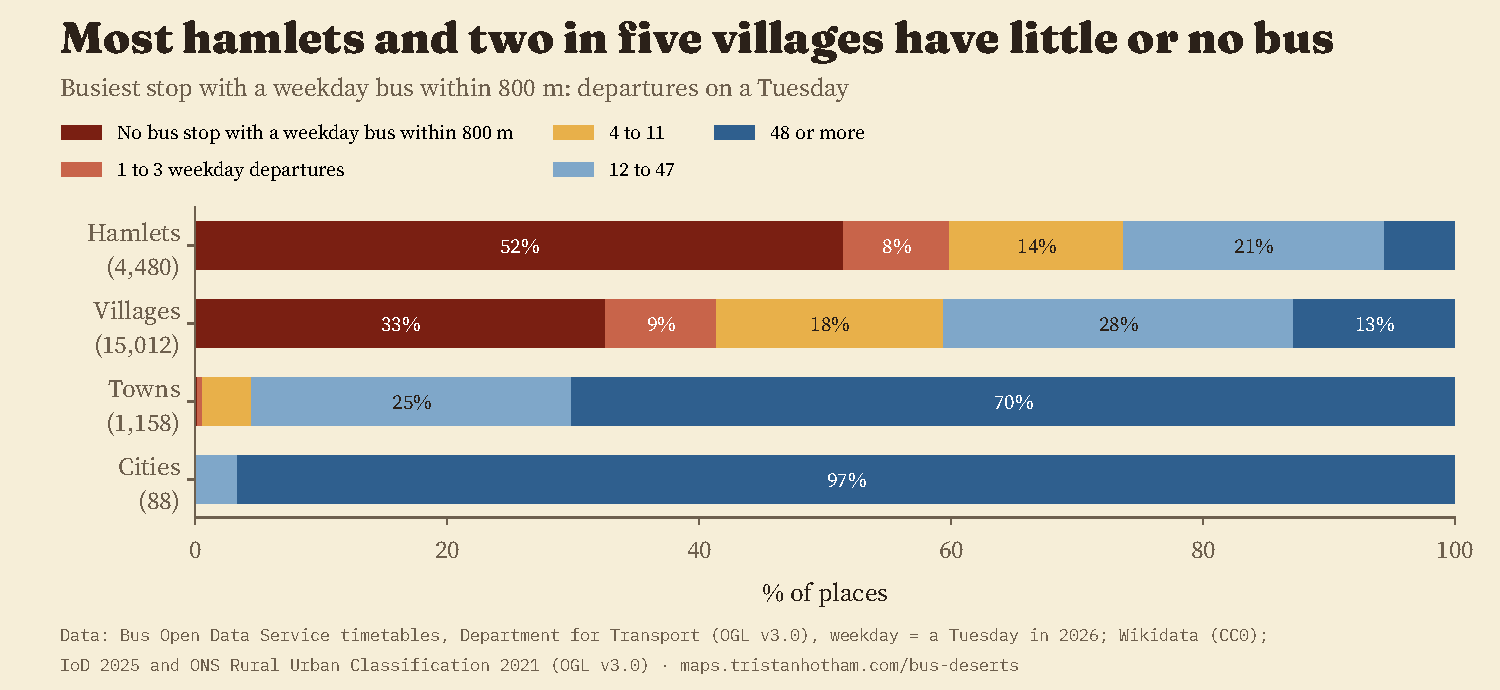
\includegraphics[width=\textwidth]{f_classes.pdf}\caption{Service within 800 m by settlement type. Categories are the weekday departures at the busiest stop within 800 m; the first is no stop with a weekday bus.}\label{fig:classes}\end{figure}

Figure~\ref{fig:map} maps the villages. Bus deserts occur in every region, often within a few kilometres of villages with a frequent service on a main road; regional shares are given in Section~\ref{sec:regions}.

\begin{figure}[tbp]\centering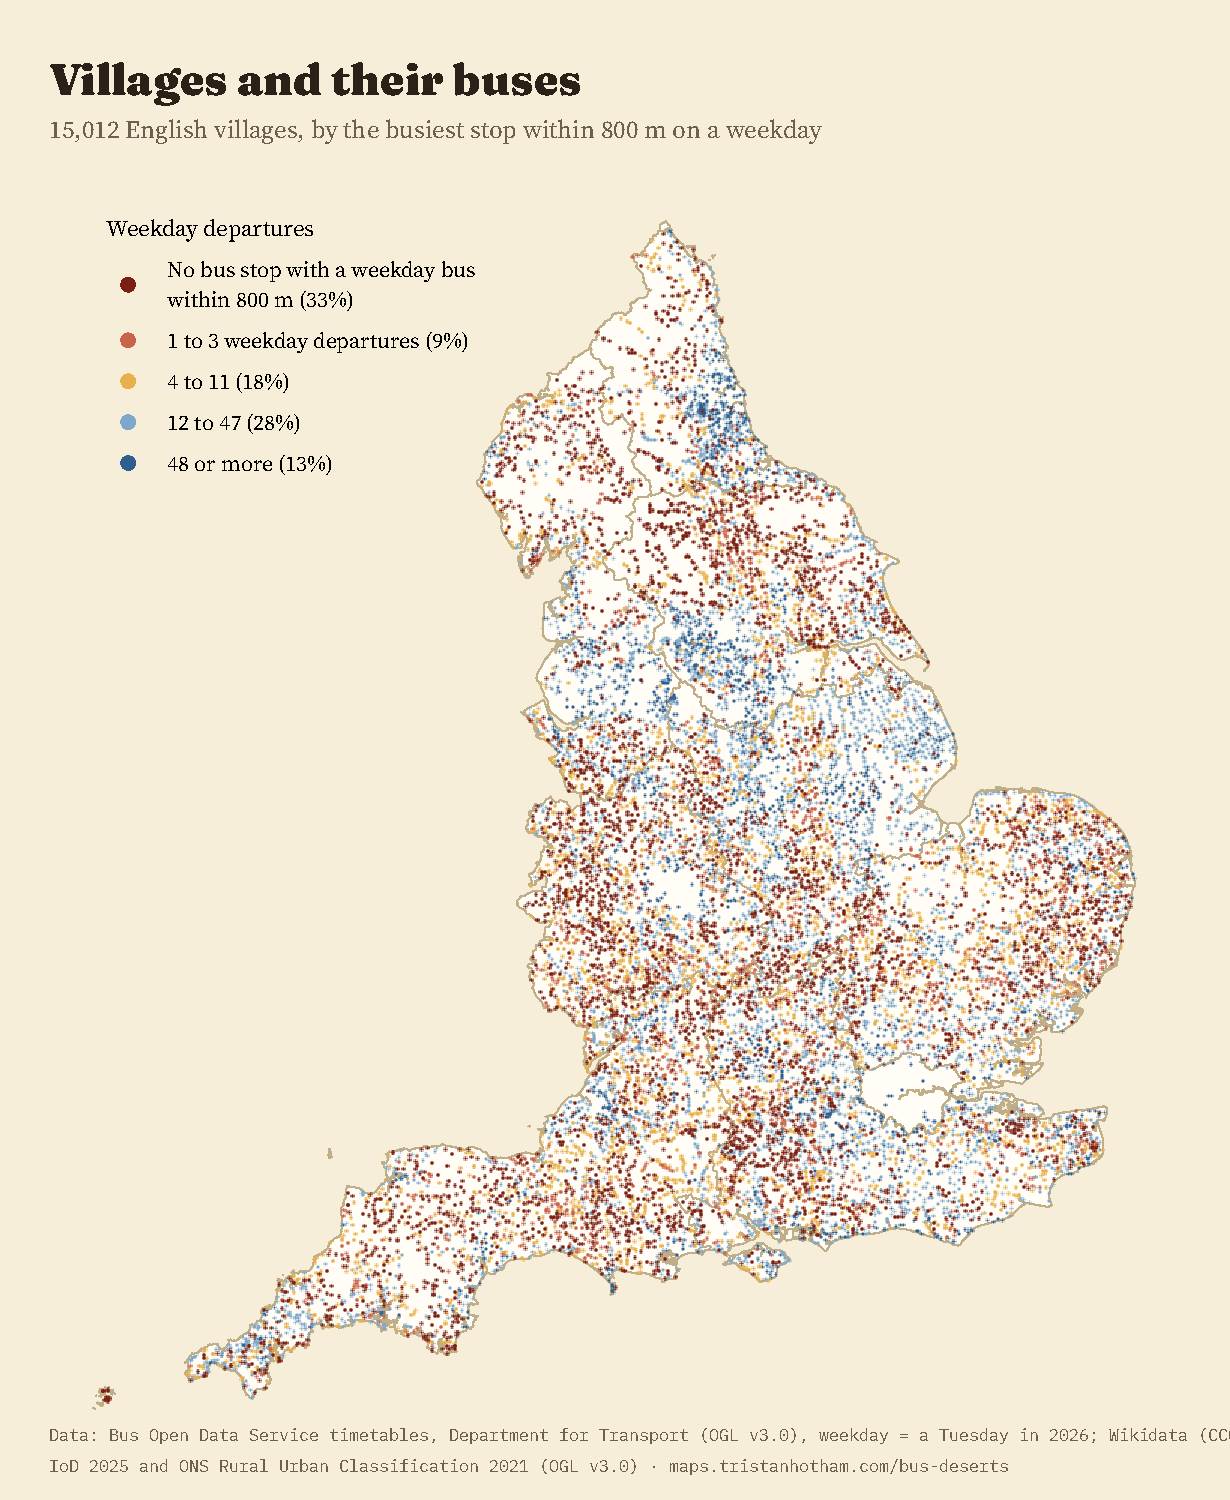
\includegraphics[width=0.82\textwidth]{f_map.pdf}\caption{English villages in Wikidata coloured by the weekday departures at the busiest stop within 800 m.}\label{fig:map}\end{figure}

\subsection{The last bus home}
Time of day sharpens the picture (Figure~\ref{fig:last}). Of the 10,119 villages with any weekday bus within 800 m, the last bus leaves before 19:00 in 4,342 (42.9\%); the median last departure is 19:24. A second group, 3,396 villages (33.6\%), lie on routes with a departure from 22:00, often on trunk routes between towns. Across all villages, 61.5\% have no bus from 19:00, 40.6\% none on the Saturday and 67.8\% none on the Sunday. Among villages with a usable weekday service, 34.6\% lack an evening bus and 46.0\% a Sunday bus, while almost all (4.7\% without) have a Saturday bus. Only 4,470 villages (29.8\%) have a usable weekday service, an evening bus and a Sunday bus together. As an exploratory description, the share of villages with a bus still to come falls from 53.1\% at 18:00 to 38.5\% at 19:00 and 25.1\% at 21:00, while the share of all served stops with a bus still to come falls more slowly, to 54.0\% at 21:00.

\begin{figure}[tbp]\centering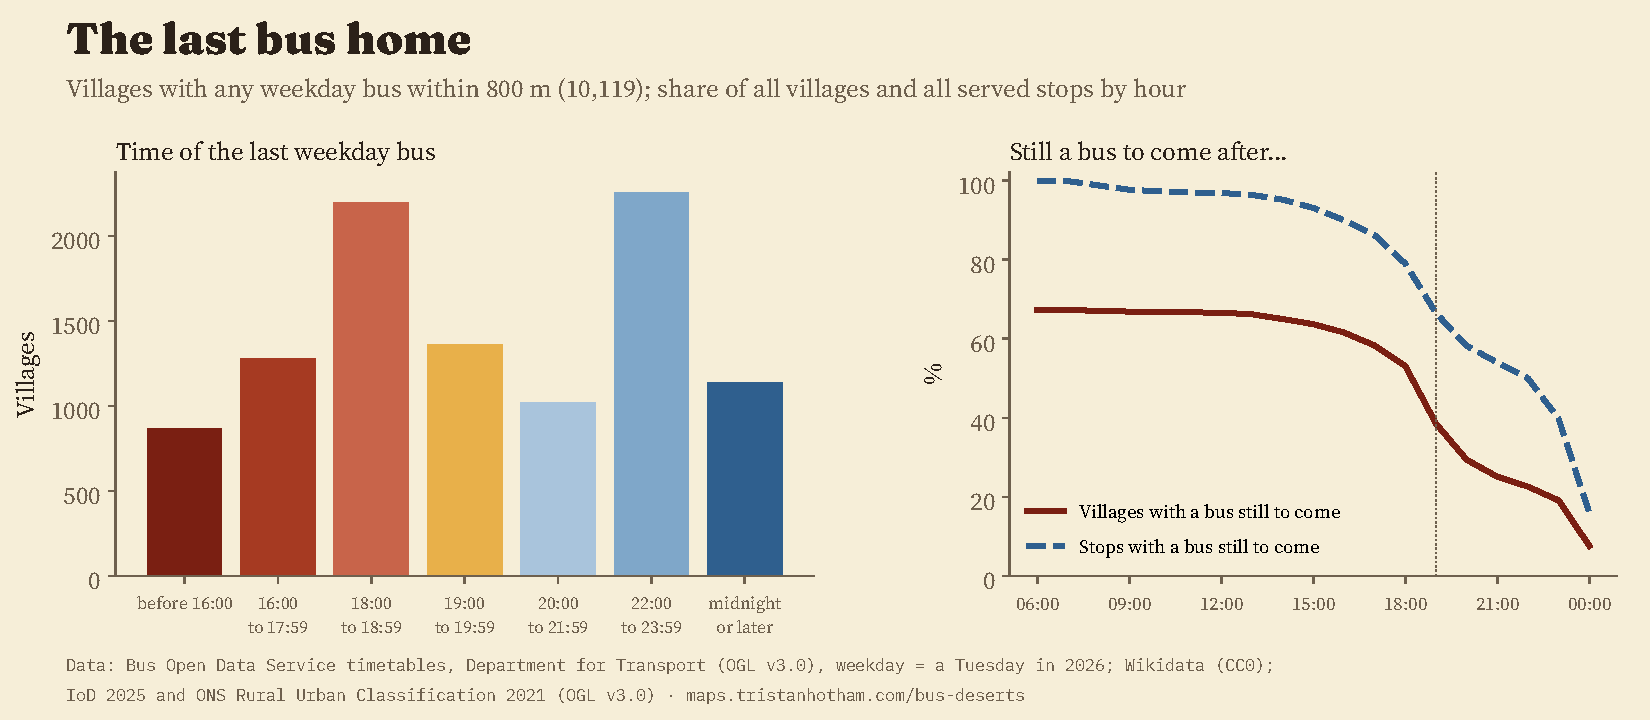
\includegraphics[width=\textwidth]{f_lastbus.pdf}\caption{Left: time of the last weekday departure from stops within 800 m, villages with any weekday bus. Right: share of all villages, and of all served stops, with a departure at or after each hour (exploratory).}\label{fig:last}\end{figure}

\subsection{Who lives beyond the network}
Turning from places to people, 5,973,411 people (10.5\% of England's population) live in 3,451 small areas without a usable weekday bus within 800 m of the area's point, and 5,283,801 (9.3\%) in areas that are bus deserts. With the geometric centroid instead, the population share is 9.8\%. 15.6\% of the population have no evening bus within 800 m and 18.5\% no Sunday bus. Among people aged 60 and over the share without a usable weekday bus is 14.1\% (1,972,418 people).

The gap is overwhelmingly rural (Table~\ref{tab:ruc}, Figure~\ref{fig:rural}). In rural small areas 45.5\% of residents have no usable weekday bus; in urban areas 3.5\%. Rural areas hold 72\% of all residents without a usable bus. The share rises from 3.2\% in urban areas near a major town to 70.3\% in smaller rural areas far from one, where 85.3\% have no evening bus and 88.4\% no Sunday bus.

\begin{table}[tbp]\centering\footnotesize\caption{Small areas by 2021 rural-urban class: residents (millions), share aged 60 and over, and population-weighted shares (\%) without a served stop within 800 m (desert), without a usable weekday bus, without an evening bus and without a Sunday bus.}\label{tab:ruc}\begin{tabular}{lrrrrrrr}\toprule Class & LSOAs & Residents (m) & Aged 60+ & Desert & No usable & No evening & No Sunday\\\midrule
Urban, near city & 26,199 & 44.29 & 22.3 & 2.7 & 3.2 & 6.2 & 8.2\\
Urban, far from city & 2,002 & 3.32 & 28.9 & 6.7 & 7.6 & 17.3 & 20.3\\
Larger rural, near city & 2,038 & 3.47 & 30.6 & 23.8 & 27.0 & 37.6 & 46.6\\
Larger rural, far from city & 849 & 1.45 & 35.2 & 26.3 & 30.1 & 47.4 & 55.0\\
Smaller rural, near city & 1,684 & 2.89 & 33.6 & 54.6 & 60.9 & 75.5 & 81.2\\
Smaller rural, far from city & 983 & 1.69 & 38.2 & 64.0 & 70.3 & 85.3 & 88.4\\
\bottomrule\end{tabular}\end{table}

\begin{figure}[tbp]\centering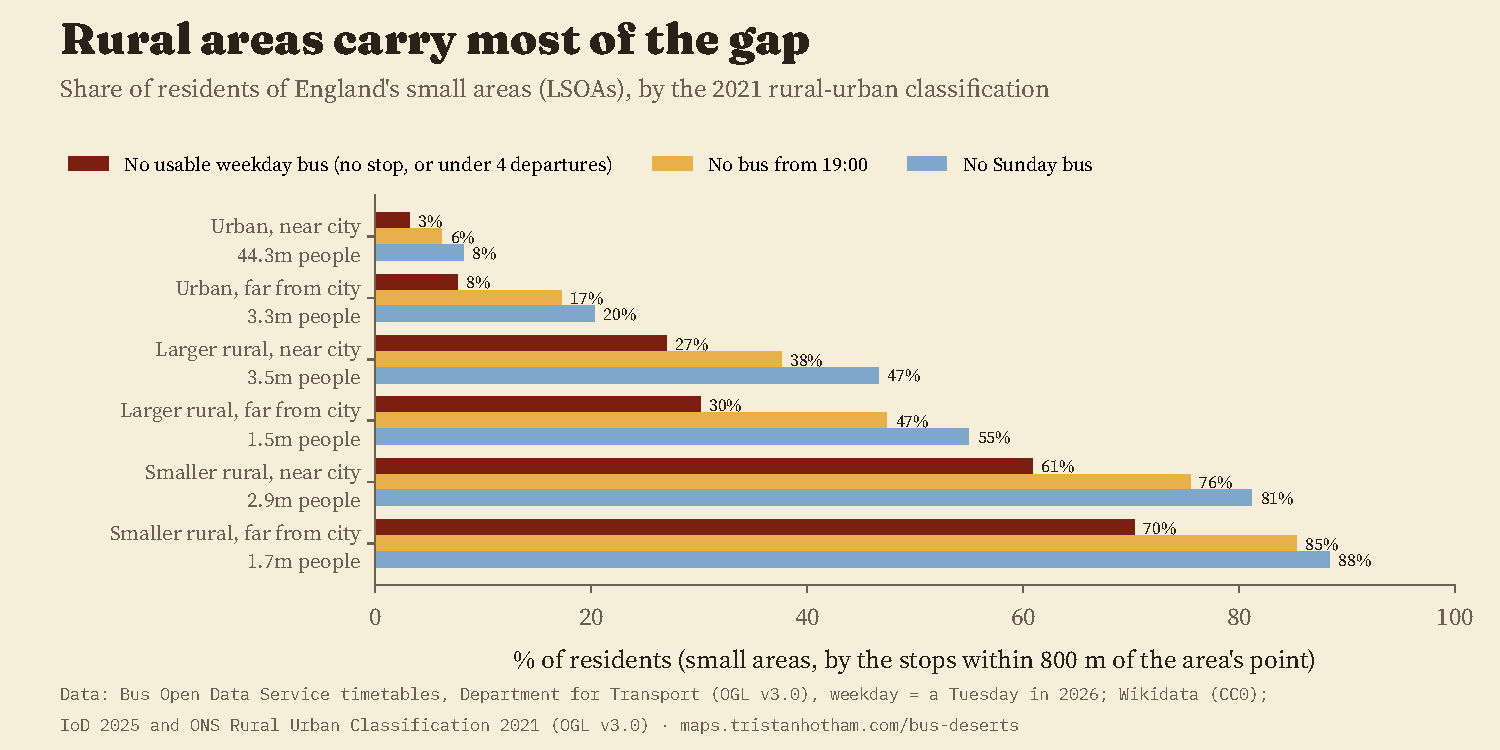
\includegraphics[width=\textwidth]{f_rural.pdf}\caption{Share of residents without a usable weekday bus, an evening bus or a Sunday bus within 800 m, by the 2021 Rural Urban Classification of their small area.}\label{fig:rural}\end{figure}

Table~\ref{tab:main} gives the planned model. H3a is supported: compared with urban areas near a major town, the odds of having no usable weekday bus are 7.1 times as high in larger rural areas near a town and 45.8 times as high in smaller rural areas far from one (average marginal effect 23.3 percentage points). H3b is supported in direction: with rurality and region fixed, a standard deviation higher deprivation score goes with lower odds of having no usable bus (odds ratio 0.68, 95\% CI 0.60 to 0.78; marginal effect -2.32 points). H3c is supported: a standard deviation higher share of residents aged 60 and over goes with higher odds (odds ratio 1.28, 1.19 to 1.38; marginal effect 1.51 points). The model's pseudo-$R^2$ is 0.35.

\begin{table}[tbp]\centering\small\caption{Planned model: logit of having no usable weekday bus within 800 m, LSOAs in England. Reference class: urban, nearer a major town or city. Region fixed effects included. Standard errors clustered by local authority district (296). N = 33,755; mean outcome 10.2\%; pseudo-$R^2$ 0.35. AME: average marginal effect in percentage points.}\label{tab:main}\begin{tabular}{lllr}\toprule Term & Odds ratio [95\% CI] & AME [95\% CI] & $p$\\\midrule
Urban, far from city & 1.75 [1.27, 2.42] & 3.41 [1.48, 5.35] & $<$0.001\\
Larger rural, near city & 7.05 [5.95, 8.36] & 11.91 [11.04, 12.78] & $<$0.001\\
Larger rural, far from city & 8.31 [6.51, 10.60] & 12.91 [11.62, 14.20] & $<$0.001\\
Smaller rural, near city & 29.39 [24.27, 35.58] & 20.61 [19.57, 21.65] & $<$0.001\\
Smaller rural, far from city & 45.84 [34.23, 61.37] & 23.32 [21.68, 24.96] & $<$0.001\\
IMD score (per SD) & 0.68 [0.60, 0.78] & -2.32 [-3.08, -1.55] & $<$0.001\\
Share aged 60+ (per SD) & 1.28 [1.19, 1.38] & 1.51 [1.04, 1.97] & $<$0.001\\
\bottomrule\end{tabular}\end{table}

Descriptively, the relation with deprivation is not a simple slope (Figure~\ref{fig:dep}). In rural small areas the share without a usable bus is 12.9\% in the most deprived decile, rises to more than half in the middle deciles and falls to 24.3\% in the least deprived. In urban areas it stays below 7\% in every decile. Why the most and least deprived rural areas are better served than the middle is not something this design can answer.

\begin{figure}[tbp]\centering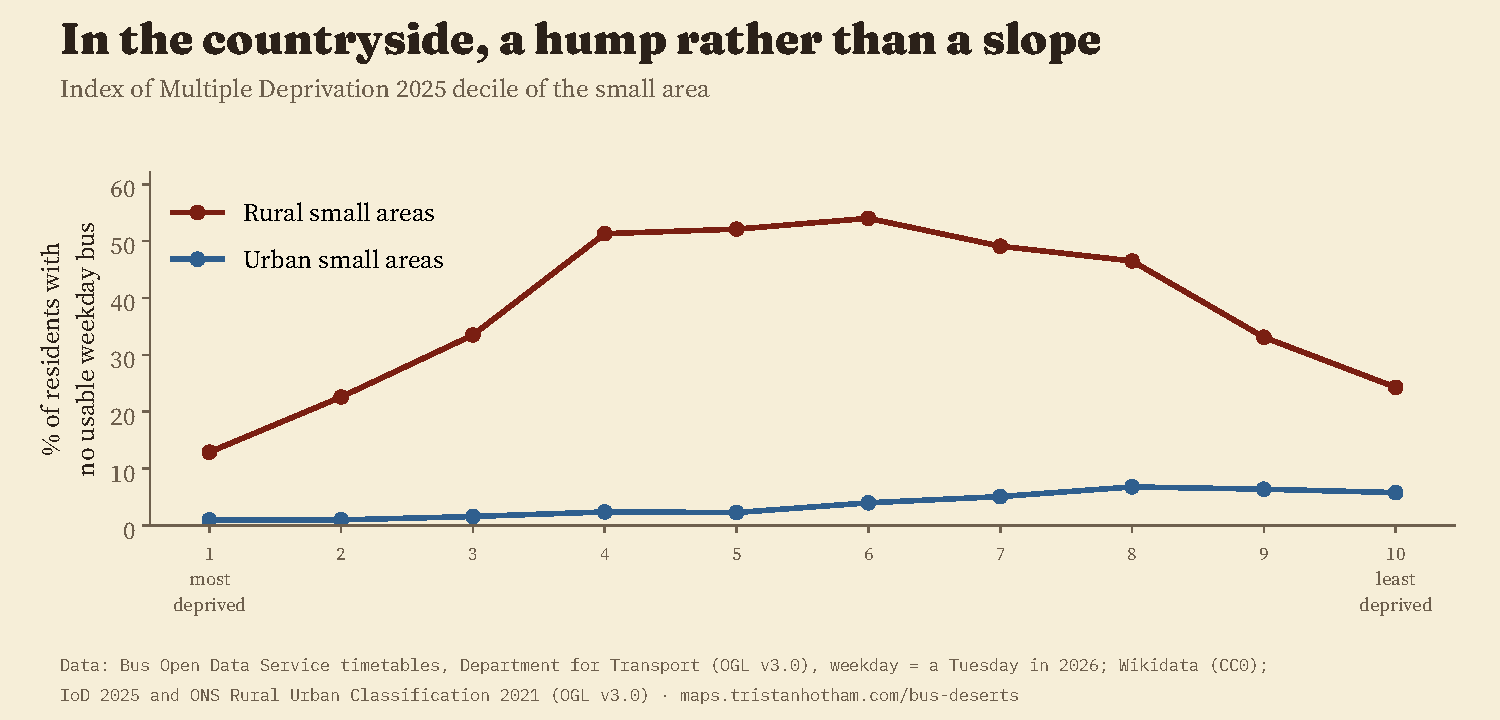
\includegraphics[width=\textwidth]{f_deprivation.pdf}\caption{Share of residents without a usable weekday bus, by IMD 2025 decile of the small area, rural and urban small areas separately.}\label{fig:dep}\end{figure}

\subsection{Regions}\label{sec:regions}
Table~\ref{tab:regions} in the appendix and Figure~\ref{fig:regions} compare regions. England has 260 weekday stop departures per 1,000 residents and London 473. Outside London the figure ranges from 425 in the West Midlands to 146 in the East of England. Stop departures depend on stop spacing as well as on service, so these are comparisons of supply on the timetable, not of buses run. The share of villages without a usable weekday bus ranges from 28.6\% in the North East to 50.3\% in the West Midlands. The West Midlands has both the highest departures per resident outside London and the highest share of villages without a usable bus: dense urban networks and thin rural ones sit side by side in the same region.

\begin{figure}[tbp]\centering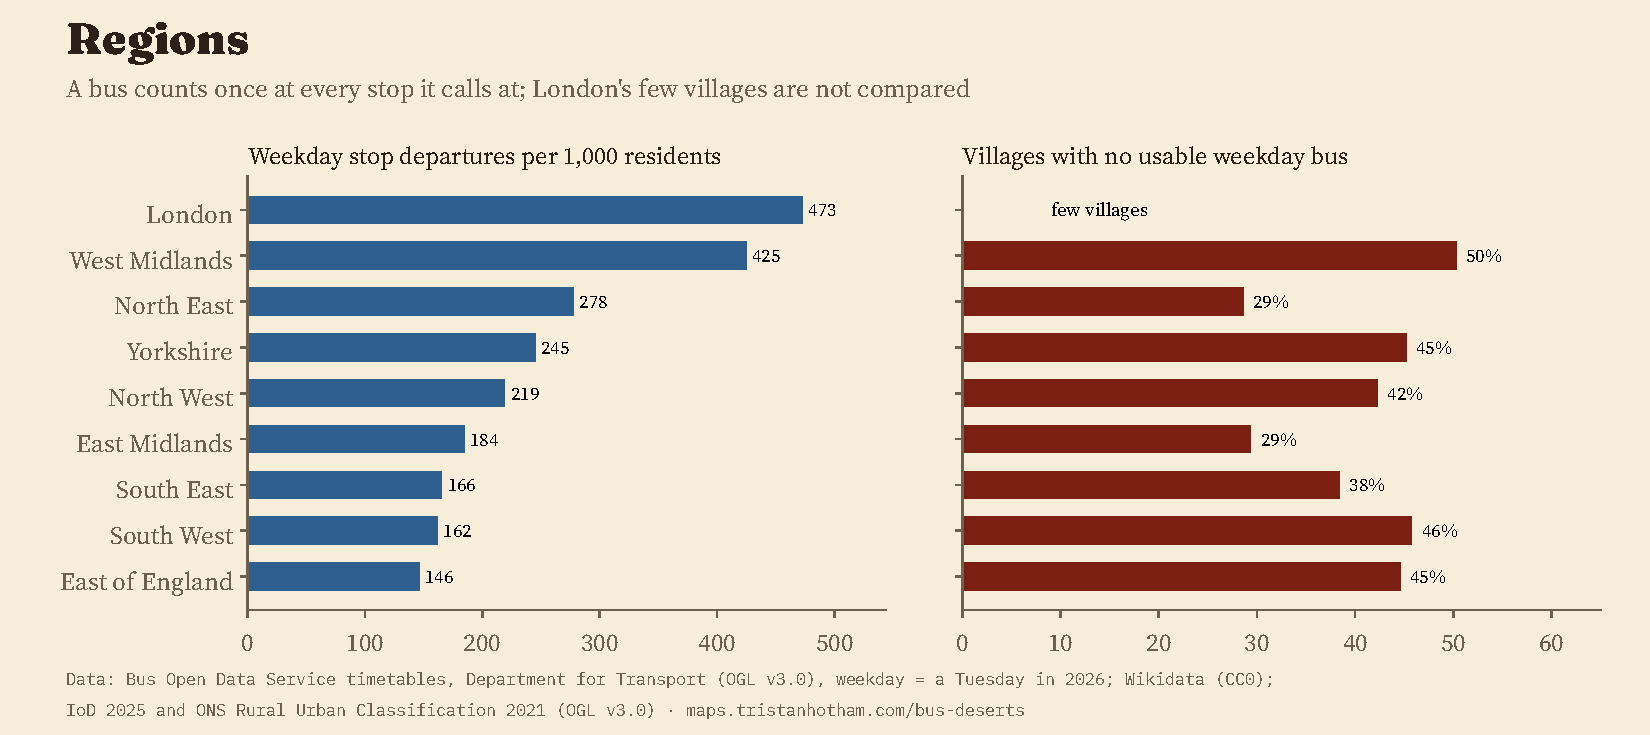
\includegraphics[width=\textwidth]{f_regions.pdf}\caption{Weekday stop departures per 1,000 residents (left) and share of villages without a usable weekday bus (right), by ONS region. London has only 25 villages in Wikidata and is not compared on the right.}\label{fig:regions}\end{figure}

\section{Robustness and falsification}\label{sec:robust}
Table~\ref{tab:robust} and Figure~\ref{fig:checks} report every planned check. The village shares move with the catchment, as they must: with 400 m, 43.8\% of villages are bus deserts; with 1,200 m, 25.9\%. With a token threshold of two departures, 3.9\% of villages have token service; with six, 14.5\%. Including tram, metro, rail and ferry stops leaves the village desert share at 32.6\%, and summing duplicated stops gives 41.0\% of villages without a usable bus (against 41.4\%).

In the small-area model the odds ratio for the share aged 60 and over stays between 1.19 and 1.41 in every logit check, and between 1.25 and 1.34 when each region is left out in turn (Table~\ref{tab:loo}). The odds ratio for deprivation stays below one in every check of the IMD, from 0.57 to 0.91, and between 0.67 and 0.70 when each region is left out. The income score gives an odds ratio of 0.54. Two results qualify H3b. First, splitting the outcome shows that the deprivation association comes from distance: for bus deserts alone the odds ratio is 0.66, but among small areas with a served stop within 800 m, deprivation is not associated with token service (odds ratio 0.91, 95\% CI 0.59 to 1.41). Second, the falsification test fails. The Indoors living environment score, which should be unrelated to buses once rurality is held fixed, has an odds ratio of 1.23 (1.14 to 1.33). Poor condition and low energy performance are more common in older, off-gas-grid rural housing, so this most likely shows that the six-class rural-urban classification leaves real differences in remoteness and density within each class. When the IMD and the Indoors score enter together the IMD odds ratio is 0.57, so the deprivation association does not disappear, but neither it nor the age association should be read as net of rurality.

\begin{table}[tbp]\centering\footnotesize\caption{Planned checks: odds ratios (95\% CI) per standard deviation for deprivation and for the share aged 60 and over. The linear probability model reports percentage-point effects. All models include the rural-urban class and region fixed effects; standard errors clustered by district.}\label{tab:robust}\begin{tabular}{p{5.4cm}p{5.1cm}lr}\toprule Check & Deprivation & Aged 60+ & N\\\midrule
Main specification & IMD 0.68 [0.60, 0.78] & 1.28 [1.19, 1.38] & 33,755\\
Radius 400 m & IMD 0.67 [0.61, 0.72] & 1.24 [1.17, 1.31] & 33,755\\
Radius 1,200 m & IMD 0.78 [0.68, 0.90] & 1.22 [1.11, 1.34] & 33,755\\
Token threshold 2 departures & IMD 0.67 [0.61, 0.73] & 1.25 [1.16, 1.35] & 33,755\\
Token threshold 6 departures & IMD 0.68 [0.57, 0.80] & 1.29 [1.19, 1.39] & 33,755\\
Tram, metro, rail and ferry stops included & IMD 0.68 [0.60, 0.77] & 1.28 [1.19, 1.38] & 33,755\\
Cross-feed duplicates summed & IMD 0.69 [0.60, 0.78] & 1.28 [1.18, 1.38] & 33,755\\
LSOA geometric centroid & IMD 0.66 [0.57, 0.76] & 1.27 [1.18, 1.37] & 33,755\\
Income deprivation instead of IMD & Income 0.54 [0.47, 0.62] & 1.19 [1.10, 1.28] & 33,755\\
Linear probability model & -1.06 [-1.50, -0.63] pp & 1.51 [1.05, 1.98] pp & 33,755\\
London excluded & IMD 0.69 [0.60, 0.78] & 1.27 [1.18, 1.37] & 28,761\\
Outcome: no served stop within 800 m & IMD 0.66 [0.60, 0.72] & 1.23 [1.14, 1.33] & 33,755\\
Outcome: token service (LSOAs with a stop) & IMD 0.91 [0.59, 1.41] & 1.41 [1.21, 1.64] & 30,705\\
Falsification: Indoors sub-domain instead of IMD & Indoors 1.23 [1.14, 1.33] & 1.41 [1.31, 1.53] & 33,755\\
IMD and Indoors sub-domain together & IMD 0.57 [0.49, 0.66]; Indoors 1.42 & 1.23 [1.13, 1.33] & 33,755\\
\bottomrule\end{tabular}\end{table}

\begin{figure}[tbp]\centering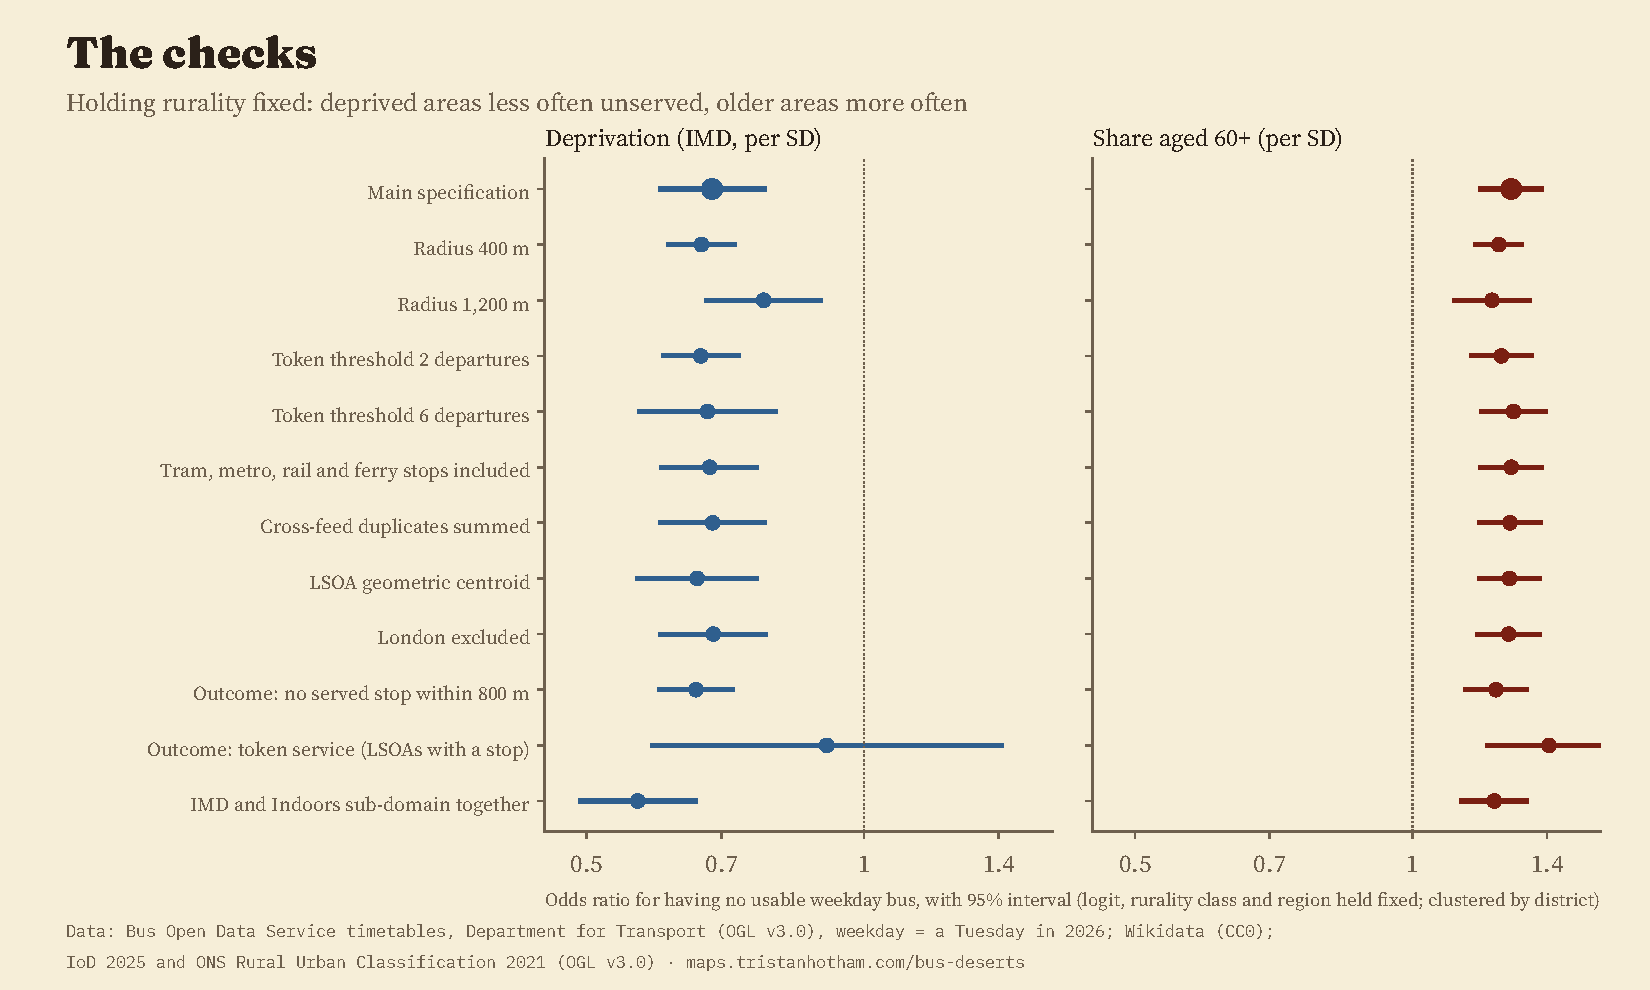
\includegraphics[width=\textwidth]{f_checks.pdf}\caption{Odds ratios for the IMD score and the share aged 60 and over in each planned check (logit; 95\% CI; standard errors clustered by district).}\label{fig:checks}\end{figure}

\section{Discussion}\label{sec:disc}
\subsection{What the pattern says}
Three findings stand out. The first is scale: two in five English villages in Wikidata have no stop with four or more weekday buses within 800 m, and one in three has no bus on a Tuesday at all within that distance. The second is that time of day is as large a gap as distance. Even where a village has a usable weekday service, a third have nothing from 19:00 and nearly half nothing on Sunday, so evening work, education and leisure, and weekend travel, are out of reach by bus for most villages. This is the time-based exclusion of \citet{church2000} and the time-dependent gap of \citet{fransen2015}, measured nationally. The third is who is affected. The people without a usable bus are mostly rural, and within the countryside they are not the most deprived: deprived rural places are more often on a bus route. This is consistent with services that follow demand and with the policy concern, in the rural literature, about older residents in car-dependent villages \citep{shergold2012}: small areas with more residents aged 60 and over are more often without a usable bus.

The deprivation pattern fits work on transport poverty that stresses the combination of low income and lack of alternatives \citep{lucas2016,mattioli2017}. It suggests that, for buses at least, the problem in rural England is less one of deprived places being left out than of whole classes of small places having no service, with the households there that lack a car carrying the cost.

\subsection{What a usable bus would take}
A simple calculation shows the scale of the time gap. Villages with a usable weekday service but no evening bus number 3,047, and those with a usable weekday service but no Sunday bus number 4,048. For many of them the missing service is not a new route but an extra journey or two at the end of the day or a Sunday timetable on an existing route. For the 4,891 villages without any stop with a weekday bus within 800 m, the question is different: either a route must divert, or the village depends on demand-responsive or community transport, which the timetable files may not show. The data cannot say which villages have such services, or what they would cost, but they identify where the gaps are in a form that can be updated as timetables change.

The regional contrast also matters for policy. Measures that average across a region, such as bus mileage or stop departures per resident, can rise while rural coverage falls, because the busiest urban corridors dominate the totals. The West Midlands illustrates this: it has the most stop departures per resident outside London and also the highest share of villages without a usable bus. Place-level measures such as those here show the distribution behind the average.

\subsection{Limitations}
The measurement rests on one week's timetables. Services that run only on school days, on market days or in summer may be missing or appear with odd times. Demand-responsive services and community transport are often not in the timetable files at all, and several English authorities rely on them in exactly the places identified here as deserts \citep{mulley2009,gray2006}; a village without a timetabled bus may have a dial-a-ride service. A few places, such as Hawes, have stops in the files but no trips on the days counted; across England 5,432 bus stops (2.2\%) have no Tuesday departure. Some of these are genuine, some are gaps in the files. Distances are straight lines, not walking routes, and the 800 m catchment ignores hills, footpaths and the absence of pavements on rural roads. A stop departure is a bus calling, not a journey to somewhere useful, so the measures say nothing about destinations or journey times, which accessibility models capture better \citep{geurs2004}. Wikidata's coverage of villages and hamlets is uneven and its points vary in precision; the small-area analysis does not depend on it. The small-area points are not population-weighted. Finally, the model is correlational and its falsification test fails, so the associations with deprivation and age describe where services are, not what causes them.

\subsection{Implications}
The measurement is cheap to repeat. Because BODS timetables are published continuously, the same code can be run on later files to track whether the counts in this paper rise or fall, which neither aggregate mileage statistics nor counts of withdrawn routes can do place by place. It also suggests where better data would help most: demand-responsive and community services in the open data, population-weighted points for small areas, and walking distances.

\section{Conclusion}\label{sec:conc}
Using every timetabled bus departure in England on one weekday, Saturday and Sunday, this paper finds that 41\% of villages have no usable weekday bus within 800 m, 62\% have no evening bus and 68\% no Sunday bus, and that 6.0 million people live in small areas without a usable weekday service, most of them in the countryside. With rurality and region held fixed, more deprived small areas are less often without a usable bus and those with older populations more often, but a planned falsification test failed, so these are descriptive patterns, not causes. The results set a reproducible baseline against which future timetables can be measured.

\section*{Data availability statement}
Data and code: Zenodo DOI https://doi.org/10.5281/zenodo.24116216. The archive contains the stop-level counts, the settlement and small-area measures, the regional and model tables, the analysis plan and all code. Interactive map: \url{https://maps.tristanhotham.com/bus-deserts/}.

\section*{AI statement}
I wrote the text, with drafting and editing assistance from Claude (Anthropic), which also helped prepare the analysis code. I reviewed and checked all text and results.

\begin{thebibliography}{99}
\bibitem[Bus Open Data Service(2026)]{bods2026} Department for Transport (2026) \textit{Bus Open Data Service}: regional timetable data in GTFS format (East Anglia, East Midlands, London, North East, North West, South East, South West, West Midlands, Yorkshire). data.bus-data.dft.gov.uk, retrieved 2026. Open Government Licence v3.0.
\bibitem[Cameron and Miller(2015)]{cameron2015} Cameron, A. C. and Miller, D. L. (2015) A practitioner's guide to cluster-robust inference. \textit{Journal of Human Resources} 50(2), 317 to 372.
\bibitem[Campaign for Better Transport(2013)]{cbt2013} Campaign for Better Transport (2013) \textit{Buses in Crisis}. London: Campaign for Better Transport.
\bibitem[Campaign for Better Transport(2018)]{cbt2018} Campaign for Better Transport (2018) \textit{Buses in Crisis: a report on bus funding across England and Wales 2010 to 2018}. London: Campaign for Better Transport.
\bibitem[Church et al.(2000)]{church2000} Church, A., Frost, M. and Sullivan, K. (2000) Transport and social exclusion in London. \textit{Transport Policy} 7(3), 195 to 205.
\bibitem[Currie(2010)]{currie2010} Currie, G. (2010) Quantifying spatial gaps in public transport supply based on social needs. \textit{Journal of Transport Geography} 18(1), 31 to 41.
\bibitem[Daniels and Mulley(2013)]{daniels2013} Daniels, R. and Mulley, C. (2013) Explaining walking distance to public transport: the dominance of public transport supply. \textit{Journal of Transport and Land Use} 6(2), 5 to 20. doi:10.5198/jtlu.v6i2.308.
\bibitem[Delbosc and Currie(2011)]{delbosc2011} Delbosc, A. and Currie, G. (2011) The spatial context of transport disadvantage, social exclusion and well-being. \textit{Journal of Transport Geography} 19(6), 1130 to 1137.
\bibitem[Department for Transport(2021)]{dft2021} Department for Transport (2021) \textit{Bus Back Better: National Bus Strategy for England}. London: Department for Transport.
\bibitem[Department for Transport(2025)]{dft2025} Department for Transport (2025) \textit{Annual Bus Statistics: Year Ending March 2025}. Accredited official statistics, first published 2025, revised 2026.
\bibitem[El-Geneidy et al.(2014)]{elgeneidy2014} El-Geneidy, A., Grimsrud, M., Wasfi, R., T\'etreault, P. and Surprenant-Legault, J. (2014) New evidence on walking distances to transit stops: identifying redundancies and gaps using variable service areas. \textit{Transportation} 41(1), 193 to 210.
\bibitem[Farrington and Farrington(2005)]{farrington2005} Farrington, J. and Farrington, C. (2005) Rural accessibility, social inclusion and social justice: towards conceptualisation. \textit{Journal of Transport Geography} 13(1), 1 to 12.
\bibitem[Fransen et al.(2015)]{fransen2015} Fransen, K., Neutens, T., Farber, S., De Maeyer, P., Deruyter, G. and Witlox, F. (2015) Identifying public transport gaps using time-dependent accessibility levels. \textit{Journal of Transport Geography} 48, 176 to 187.
\bibitem[Geurs and van Wee(2004)]{geurs2004} Geurs, K. T. and van Wee, B. (2004) Accessibility evaluation of land-use and transport strategies: review and research directions. \textit{Journal of Transport Geography} 12(2), 127 to 140.
\bibitem[geographr(2026)]{geographr} humaniverse (2026) \textit{geographr}: R package of UK geographic boundaries, lookups and classifications (\texttt{ruc21\_lsoa21}, \texttt{boundaries\_lsoa21}). GitHub, github.com/humaniverse/geographr, retrieved 2026. Data from the Office for National Statistics, Open Government Licence v3.0.
\bibitem[Gray et al.(2006)]{gray2006} Gray, D., Shaw, J. and Farrington, J. (2006) Community transport, social capital and social exclusion in rural areas. \textit{Area} 38(1), 89 to 98. doi:10.1111/j.1475-4762.2006.00662.x.
\bibitem[Lucas(2012)]{lucas2012} Lucas, K. (2012) Transport and social exclusion: where are we now? \textit{Transport Policy} 20, 105 to 113.
\bibitem[Lucas et al.(2016)]{lucas2016} Lucas, K., Mattioli, G., Verlinghieri, E. and Guzman, A. (2016) Transport poverty and its adverse social consequences. \textit{Proceedings of the Institution of Civil Engineers: Transport} 169(6), 353 to 365. doi:10.1680/jtran.15.00073.
\bibitem[Mattioli(2014)]{mattioli2014} Mattioli, G. (2014) Where sustainable transport and social exclusion meet: households without cars and car dependence in Great Britain. \textit{Journal of Environmental Policy and Planning} 16(3), 379 to 400. doi:10.1080/1523908X.2013.858592.
\bibitem[Mattioli et al.(2017)]{mattioli2017} Mattioli, G., Lucas, K. and Marsden, G. (2017) Transport poverty and fuel poverty in the UK: from analogy to comparison. \textit{Transport Policy} 59, 93 to 105.
\bibitem[MHCLG(2025)]{iod2025} Ministry of Housing, Communities and Local Government (2025) \textit{The English Indices of Deprivation 2025}: statistical release, technical report and File 7 (all ranks, scores, deciles and population denominators). Accredited official statistics. Open Government Licence v3.0.
\bibitem[Mulley and Nelson(2009)]{mulley2009} Mulley, C. and Nelson, J. D. (2009) Flexible transport services: a new market opportunity for public transport. \textit{Research in Transportation Economics} 25(1), 39 to 45.
\bibitem[ONS(2026)]{ons2021ruc} Office for National Statistics (2026) \textit{2021 Rural Urban Classification}. Methodology and LSOA classification, updated 2026. Open Government Licence v3.0.
\bibitem[Pereira et al.(2017)]{pereira2017} Pereira, R. H. M., Schwanen, T. and Banister, D. (2017) Distributive justice and equity in transportation. \textit{Transport Reviews} 37(2), 170 to 191.
\bibitem[Seabold and Perktold(2010)]{seabold2010} Seabold, S. and Perktold, J. (2010) Statsmodels: econometric and statistical modeling with Python. \textit{Proceedings of the 9th Python in Science Conference}, 92 to 96.
\bibitem[Shergold and Parkhurst(2012)]{shergold2012} Shergold, I. and Parkhurst, G. (2012) Transport-related social exclusion amongst older people in rural Southwest England and Wales. \textit{Journal of Rural Studies} 28(4), 412 to 421. doi:10.1016/j.jrurstud.2012.01.010.
\bibitem[Social Exclusion Unit(2003)]{seu2003} Social Exclusion Unit (2003) \textit{Making the Connections: Final Report on Transport and Social Exclusion}. London: Office of the Deputy Prime Minister.
\bibitem[Transport Committee(2019)]{tc2019} House of Commons Transport Committee (2019) \textit{Bus Services in England outside London}. Ninth Report of Session 2017 to 19, HC 1425.
\bibitem[Transport Committee(2023)]{tc2023} House of Commons Transport Committee (2023) \textit{Implementation of the National Bus Strategy}. Fourth Report of Session 2022 to 23, HC 161.
\bibitem[Velaga et al.(2012)]{velaga2012} Velaga, N. R., Beecroft, M., Nelson, J. D., Corsar, D. and Edwards, P. (2012) Transport poverty meets the digital divide: accessibility and connectivity in rural communities. \textit{Journal of Transport Geography} 21, 102 to 112.
\bibitem[Vrande\v{c}i\'c and Kr\"otzsch(2014)]{vrandecic2014} Vrande\v{c}i\'c, D. and Kr\"otzsch, M. (2014) Wikidata: a free collaborative knowledgebase. \textit{Communications of the ACM} 57(10), 78 to 85.
\end{thebibliography}

\appendix
\section{Appendix: further tables and data construction}
\begin{table}[htbp]\centering\footnotesize\caption{Regions: residents (millions), weekday and Sunday stop departures per 1,000 residents, population share without a usable weekday bus, villages and shares without a usable weekday bus and without a Sunday bus (not shown for London's 25 villages), and share of bus stops with no Tuesday departure.}\label{tab:regions}\begin{tabular}{lrrrrrrrr}\toprule Region & Res. (m) & Wk/1,000 & Sun/1,000 & Pop. no usable & Villages & No usable & No Sunday & Stops 0 Tue\\\midrule
London & 8.87 & 473 & 372 & 0.3 & 25 &  &  & 1.4\\
West Midlands & 6.02 & 425 & 189 & 9.4 & 1,637 & 50.3 & 80.0 & 2.2\\
North East & 2.68 & 278 & 138 & 6.4 & 859 & 28.6 & 48.7 & 1.7\\
Yorkshire & 5.54 & 245 & 124 & 10.5 & 1,727 & 45.2 & 55.1 & 1.5\\
North West & 7.52 & 219 & 102 & 8.3 & 1,222 & 42.3 & 60.0 & 1.4\\
East Midlands & 4.93 & 184 & 62 & 14.8 & 1,907 & 29.4 & 72.7 & 1.2\\
South East & 9.39 & 166 & 85 & 12.9 & 2,598 & 38.4 & 61.6 & 3.0\\
South West & 5.77 & 162 & 66 & 16.8 & 2,843 & 45.8 & 72.5 & 3.8\\
East of England & 6.40 & 146 & 46 & 17.2 & 2,194 & 44.6 & 78.2 & 2.4\\
\bottomrule\end{tabular}\end{table}
\begin{table}[htbp]\centering\small\caption{Leave one region out: odds ratios (95\% CI) from the main model with the named region dropped.}\label{tab:loo}\begin{tabular}{llll}\toprule Region left out & IMD (per SD) & Aged 60+ (per SD) & N\\\midrule
North East & 0.69 [0.60, 0.79] & 1.28 [1.19, 1.39] & 32,073\\
North West & 0.67 [0.60, 0.73] & 1.25 [1.15, 1.35] & 29,188\\
Yorkshire & 0.69 [0.60, 0.80] & 1.26 [1.17, 1.37] & 30,400\\
East Midlands & 0.68 [0.59, 0.79] & 1.30 [1.19, 1.42] & 30,908\\
West Midlands & 0.70 [0.61, 0.80] & 1.27 [1.18, 1.38] & 30,181\\
East of England & 0.68 [0.59, 0.79] & 1.34 [1.23, 1.45] & 29,997\\
London & 0.69 [0.60, 0.78] & 1.27 [1.18, 1.37] & 28,761\\
South East & 0.68 [0.59, 0.80] & 1.29 [1.18, 1.41] & 28,184\\
South West & 0.68 [0.59, 0.78] & 1.27 [1.17, 1.38] & 30,348\\
\bottomrule\end{tabular}\end{table}

\textbf{Data construction.} The reduction script counts, for each trip active on a date, a departure at every stop where passengers can board (pickup type other than 1), using the departure time or, if absent, the arrival time. Times after midnight are kept as minutes after the start of the service day (for example 25:10). The hourly counts run from hour 0 to hour 29. Stops are placed in regions and in England by their coordinates; coastal stops just outside the generalised boundaries take the nearest region within 2 km. Settlements are in England if their point is inside the generalised England boundary. The settlement hand checks are in \texttt{code/overrides.json}.

\textbf{Software.} Python 3 with pandas, numpy, scipy (k-d trees for distances), geopandas, shapely, pyproj, statsmodels, rdata (to read the geographr files), matplotlib and xelatex. All code is in the data and code archive.

\end{document}
